%# -*- coding: utf-8-unix -*-
%%==================================================
%% chapter01.tex for SJTU Master Thesis
%%==================================================

%\bibliographystyle{sjtu2}%[此处用于每章都生产参考文献]
\chapter{密钥信息泄露的应用}
\label{chap:App}
由于实际密钥信息集合中包含了和给定的子密钥集合$K$相同大小的密钥信息,因此只要其中存在密钥信息泄露,基于猜测集合$K$的攻击(这些攻击中$K$一般用来猜测一个区分器的输入/输出)就可以通过用$K$的实际密钥信息集合$K'_0$代替$K$成为猜测集合来降低其复杂度。
在本章中,我们将会介绍两种基于密钥信息泄露的AKI的应用。

\section{对TWINE-80的零相关攻击}
Yanfeng Wang等人在\citen{wang2014improved}中通过其提出的$((2,9),4,14,5)$这一区分器给出了一个对23轮TWINE-80密码的多维零相关线性攻击,而Li Lin等人在\citen{lin2016automatic}中指出了Wang在其文章中错误使用的密钥桥,并给出了一个基于区分器$((6,9),4,14,5)$的新的23轮攻击,并给出了3个密钥桥来降低其复杂度。
然而,Lin提出的密钥桥中,$RK^6_{22}\oplus S(RK^2_{22})\oplus S(RK^5_{22})\Rightarrow RK^6_2$并不能用来降低他们提出的23轮攻击,因为$RK^6_2$并不在$X^6_4$的密钥依赖路径中。
我们使用我们的AKI-最小割算法,重新分析了上述两个攻击,发现他们都可以由原来的19个密钥块组成的猜测集合降低为一个16个密钥块组成的实际密钥信息集合。
表\ref{tab:twine}展示了两种攻击的猜测集合和实际密钥信息集合。
\begin{table}[htbp]
    \centering
    \begin{tabular}{c|c|c}
        区分器 & 猜测集合 & 实际密钥信息集合\\
        \hline
        \multirow{4}{*}{((2,9),4,14,5)} & $WK^3_0|WK^4_0|WK^6_0|WK^{13}_1|WK^{15}_1$ & $WK_0^0|WK_0^3|WK_0^4|WK_0^6|WK_0^{14}$\\
                                        & $WK^6_2|WK_3^{13}|WK_{18}^{13}|WK_{19}^{15}|WK_{20}^3$ & $WK_0^{15}|WK_0^{17}|WK_0^{18}|WK_0^{19}$ \\
                                        & $WK_{20}^{16}|WK_{21}^1|WK_{21}^{13}|WK_{21}^{14}|WK_{22}^4$ & $WK^0_6|WK^0_9|WK_{10}^0$\\ 
                                        & $WK_{22}^6|WK_{22}^{13}|WK_{22}^{14}|WK_{22}^{15}$ & $WK_{13}^0|WK_{13}^{16}|WK_{19}^{16}|WK_{20}^{16}$ \\
        \hline
        \multirow{4}{*}{((6,9),4,14,5)} & $WK^3_0|WK^6_0|WK^{16}_0|WK^4_1|WK^{16}_1$ & $WK_0^0|WK_0^1|WK_0^3|WK_0^6|WK_0^7$\\
                                        & $WK^{15}_2|WK_3^{14}|WK_{18}^{13}|WK_{19}^{15}|WK_{20}^3$ & $WK_0^8|WK_0^{15}|WK_0^{16}|WK_0^{18}$ \\
                                        & $WK_{20}^{16}|WK_{21}^1|WK_{21}^{13}|WK_{21}^{14}|WK_{22}^4$ & $WK^0_6|WK_6^{16}|WK_9^0$\\ 
                                        & $WK_{22}^6|WK_{22}^{13}|WK_{22}^{14}|WK_{22}^{15}$ & $WK_{9}^{16}|WK_{13}^{16}|WK_{19}^{16}|WK_{20}^{16}$ \\
        \hline
    \end{tabular}
    \bicaption[tab:twine]{对TWINE-80的攻击的优化}{两种区分器下的19密钥块的猜测集合和16密钥块的实际密钥信息集合}{Optimization for attacks on TWINE-80}{The 19-nibble subkey set and 16-nibble AKI-set of two different distinguishers of TWINE-80}
\end{table}

\section{对RECTANGLE-128的中间相遇攻击}
本节中我们将会结合基础的中间相遇技术和RECTANGLE的密钥弱点来得出一个对RECTANGLE-128的12轮中间相遇攻击。
我们的攻击的数据复杂度只有8个已知明文,时间复杂度为$2^{126.32}$次加密,空间复杂度低于$2^{125}$个128比特分组。
在接下来的讨论中,我们认为12轮简化的RECTANGLE拥有12轮的加密方程和一个最终的白化密钥加步骤。

我们设定中间相遇的中间值$V$为第6轮中的4比特密文$X_6^0,X_6^4,X_6^8,X_6^{12}$,其计算可以分为加密和解密两种方法。
在加密方向上,计算$V$可以使用明文$X_0$和子密钥集合$K_t$;而在解密方向上,计算$V$需要用到密文$X_{12}$和子密钥集合$K_b$。

在加密方向上,6轮向前的计算路径的密钥依赖路径上共计由288比特的轮密钥,而在解密方向的6轮向后计算路径的密钥依赖路径上共计由292比特的轮密钥,即$|K_t|=288$,$|K_b|=292$。
也就是说,为了计算$X_6^0,X_6^4,X_6^8,X_6^{12}$,我们需要在前6轮加密中猜测288比特密钥,在后6轮解密中猜测292比特密钥,而这样做的代价是无法形成一个攻击的。
然而,无论是向前的路径还是向后的路径,由于RECTANGLE-128密钥编排方案的信息泄露,两者的AKI均只有124,也就是说只要124比特的子密钥就足以得出所有$K_t$或是$K_b$中所有的子密钥比特了,这样就使得12轮的中间相遇攻击变为可能。
图\ref{fig:12}展示了该攻击的计算路径和密钥依赖路径$K_t$和$K_b$,其实际密钥信息集合分别陈列在附录\ref{AppendixA}中。为了方便描述,我们记$K'_t$为$K_t$的实际密钥信息集合,相对应的$K'_b$为$K_b$的实际密钥信息集合。
\begin{figure}
\centering
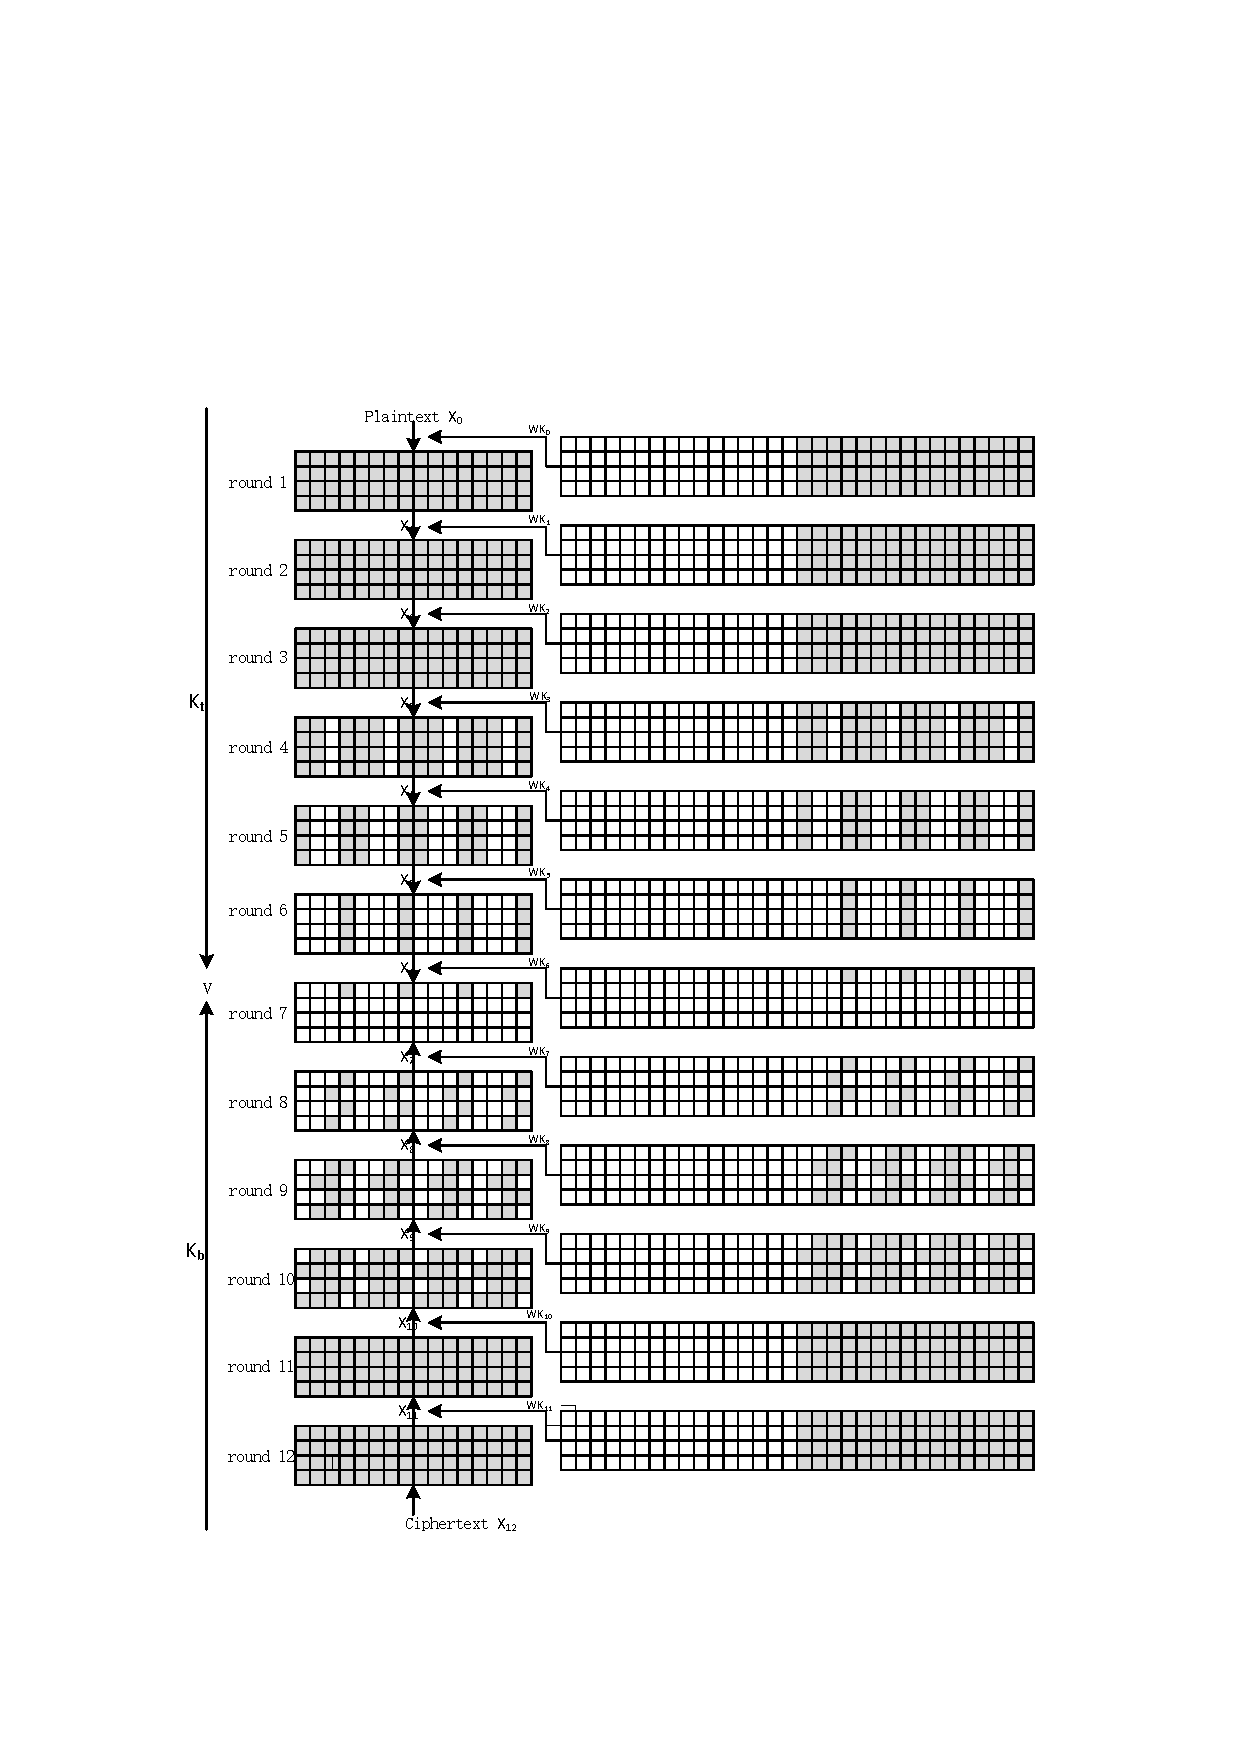
\includegraphics[width=130mm]{12.pdf}
\bicaption[fig:12]{对RECTANGLE-128的12轮中间相遇攻击}{一条6轮的前向(后向)计算路径(左)和密钥依赖路径(右)}{12-round MITM attack}{A 6-round forward (backward) Computation Path (left) and the Key Dependency Path (right).}
\end{figure}
 
在我们的攻击中,每次猜测$K'_t$(从而推出$K_t$),我们计算出相对应的$V$并将其存在一个哈希表中。
同样,每次猜测$K'_b$,计算出相应的$V$并在哈希表中寻找与他匹配的$K_t$。
如果在两个方向上的计算的出了相同的$V$,那么哈希表中将会由这样一对匹配,这个匹配所对应的密钥猜测$(K_t,K_b)$就会被认为是一个候选的密钥猜测。
算法\ref{alg:MITM}中包含了该攻击的伪代码。
\begin{algorithm}
\footnotesize
\caption{对RECTANGLE-128的12轮中间相遇攻击}
\label{alg:MITM}
\begin{algorithmic}[1]
\For {所有可能的124比特$K^{\prime}_t$的值}
\State 推测出$K_t$中的比特;
\State 将明文$P_i$加密以得到$X_6^0[i],X_6^4[i],X_6^8[i],X_6^{12}[i]$, $i=1,\dots,8$;
\State 将$K^{\prime}_t$存储到哈希表$T_1$,目录为$X_6^0[1],X_6^4[1],X_6^8[1],X_6^{12}[1]||\dots||X_6^0[8],X_6^4[8],X_6^8[8],X_6^{12}[8]$;
\EndFor
\For {所有可能的124比特$K^{\prime}_b$的值}
\State 推测出$K_b$中的比特;
\State 将明文$C_i$加密以得到$X_6^0[i],X_6^4[i],X_6^8[i],X_6^{12}[i]$, $i=1,\dots,9$;
\If {以$X_6^0[1],X_6^4[1],X_6^8[1],X_6^{12}[1]||\dots||X_6^0[8],X_6^4[8],X_6^8[8],X_6^{12}[8]$为目录的数据存在于哈希表$T_1$中}
\State 取出相对应的$K^{\prime}_t$和现有的$K^{\prime}_b$组成一个候选的蜜月猜测.
\EndIf
\EndFor
\State 枚举得到的所有的候选密钥.
\end{algorithmic}
\end{algorithm}

根据密钥编排方案,在猜测出所有$K'_t$的124比特后,$K'_b$中由92比特也可以被推出。
因此,这两条密钥依赖路径共享了92比特的密钥信息,我们就可以分离出这92比特来减少穷搜的时间复杂度。

\noindent
\textbf{复杂度分析:}在该12轮攻击中,我们使用了8个已知明密文对。攻击的时间复杂度为$\mathcal{O}(2^{124})$。
更精确的来说,在中间相遇部分共有$2^{124\cdot 8\cdot 0.5}=2^{126}$次12轮加密,剩下的候选密钥共有$2^{124+124-92-4\cdot 8}=2^{124}$个。
因此,在枚举阶段需要$2^{124}$个完整的加密。总共的时间复杂度为$2^{126.32}$次12轮RECTANGLE-128的加密过程。
空间复杂度为$\mathcal{O}(2^{124})$。更精确的来说,我们需要$2^{124}$个大小为$4\cdot 8+124=156$比特的分组,小于$2^{125}$个128比特的分组。

我们的攻击是第一个对RECTANGLE-128的拥有非常低数据复杂度的攻击。
实际上,在\citen{bouillaguet2011automatic}中也提到,为了更好的安全性理解,确定仅用非常少的可用数据最多可以攻击多少轮非常重要。
尽管这个攻击可能不是针对RECTANGLE-128最好的攻击,但是类似这种的中间相遇攻击可以非常容易地由其密钥编排方案的信息泄露得出,而这在某种程度上体现了密钥信息泄露的严重后果和AKI的重要性。
